\documentclass[12pt]{article}
\usepackage[utf8]{inputenc}
\usepackage[T1]{fontenc}
\usepackage[margin=2.5cm]{geometry}
\usepackage{graphicx}
\usepackage{tikz}
\usepackage{amsmath}
\usepackage{float}
\usepackage{parskip}

\renewcommand{\contentsname}{Índice}
\renewcommand{\figurename}{Figura}
\renewcommand{\tablename}{Tabla}

\newcommand{\spanishtoday}{%
  \number\day\ de \ifcase\month\or enero\or febrero\or marzo\or abril\or mayo\or
  junio\or julio\or agosto\or septiembre\or octubre\or noviembre\or diciembre\fi
  \ de \number\year
}

\emergencystretch=3em

\newcommand{\kmapii}[4][]{%
\begin{tikzpicture}[scale=1.0, every node/.style={font=\small}]
  \draw (0,0) grid (2,2);
  \node at (1, 2.75) {$#2$};
  \node[rotate=90] at (-1.1, 1) {$#3$};
  \foreach \lbl [count=\i from 0] in {0,1}
    \node at (\i+0.5, 2.3) {\lbl};
  \foreach \lbl [count=\j from 0] in {0,1}
    \node at (-0.4, 1.5-\j) {\lbl};
  \foreach \v [count=\k from 0] in {#4} {
    \pgfmathtruncatemacro{\col}{mod(\k,2)}
    \pgfmathtruncatemacro{\row}{div(\k,2)}
    \node at (\col+0.5, 1.5-\row) {\v};
  }
  #1
\end{tikzpicture}%
}

\newcommand{\kmapiv}[4][]{%
\begin{tikzpicture}[scale=1.0, every node/.style={font=\small}]
  \draw (0,0) grid (4,4);
  \node at (2, 4.75) {$#2$};
  \node[rotate=90] at (-1.1, 2) {$#3$};
  \foreach \lbl [count=\i from 0] in {00,01,11,10}
    \node at (\i+0.5, 4.3) {\lbl};
  \foreach \lbl [count=\j from 0] in {00,01,11,10}
    \node at (-0.45, 3.5-\j) {\lbl};
  \foreach \v [count=\k from 0] in {#4} {
    \pgfmathtruncatemacro{\col}{mod(\k,4)}
    \pgfmathtruncatemacro{\row}{div(\k,4)}
    \node at (\col+0.5, 3.5-\row) {\v};
  }
  #1
\end{tikzpicture}%
}

\newcommand{\grupoii}[5]{%
  \draw[#1, very thick, rounded corners=8pt]
    (#2+0.12, 1.12-#5) rectangle (#4+0.88, 1.88-#3);
}
\newcommand{\grupo}[5]{%
  \draw[#1, very thick, rounded corners=8pt]
    (#2+0.12, 3.12-#5) rectangle (#4+0.88, 3.88-#3);
}

\begin{document}

\begin{titlepage}
    \centering
    \vspace*{1cm}

    
\includegraphics[width=8cm]{tec_logo.pdf}\\[1.5cm]

    {\large Instituto Tecnológico de Costa Rica}\\[0.3cm]
    {\large Escuela de Ingeniería en Computadores}\\[2cm]

    {\Large \textbf{CE1107: Fundamentos de Arquitectura de Computadores}}\\[0.5cm]

    \vspace{2cm}
    {\Huge \textbf{Bitácora del Proyecto}}\\[0.5cm]
    {\Large Cerrojo}\\[2cm]

    \begin{flushleft}
        \large
        \textbf{Estudiantes:}\\
        Guillermo Sánchez Cedeño\\
        Kendall Fernández Obando\\[0.5cm]
        \textbf{Profesor:} Luis Chavarría Zamora\\[0.5cm]
        \textbf{Semestre:} II Semestre 2026
    \end{flushleft}

    \vfill

    {\large \spanishtoday}

\end{titlepage}

\tableofcontents
\newpage

\section{7 de septiembre de 2026}

\subsection{Codificador de señas}

Para esta sesión trabajamos en el codificador, que es el bloque encargado de
tomar la lectura de los sensores de la mano y comprimirla a un número binario de
tres bits que el resto del circuito pueda manejar con comodidad. La idea del
proyecto es que el usuario ingrese cada dígito de la contraseña levantando una
cantidad determinada de dedos, entonces necesitamos alguna manera de traducir esa
seña a un valor numérico antes de poder guardarla o compararla.

El sistema cuenta con cuatro sensores, uno por dedo, a los que llamamos $S_1$,
$S_2$, $S_3$ y $S_4$. La seña válida es la que levanta los dedos en orden, es
decir que para representar el número tres se activan $S_1$, $S_2$ y $S_3$. Ahora
bien, nada le impide físicamente al usuario levantar una combinación que no siga
ese orden, como por ejemplo levantar únicamente el dedo del medio, pero de esos
casos no se encarga este bloque.

Para eso tenemos un verificador aparte, cuya única responsabilidad es revisar si
la seña que se está ingresando respeta el orden y avisarle al resto del sistema
cuando no lo hace. Está división de responsabilidades es la que nos permite
diseñar el codificador asumiendo que la seña que le llega ya viene bien formada,
sin tener que meterle a este bloque la lógica de validación encima.

Como tenemos cuatro sensores, en total existen 16 combinaciones posibles de
entrada, de las cuales únicamente 5 corresponden a señas válidas, que son las de
los valores del 0 al 4. Las otras 11 son las que el verificador se encarga de
rechazar.

\subsection{Tabla de verdad}

Empezamos construyendo la tabla de verdad con las cinco combinaciones válidas,
relacionando el estado de los sensores con la cantidad de dedos levantados y con
el valor binario de tres bits que le corresponde en la salida.

\begin{table}[H]
\centering
\begin{tabular}{cccc|c|ccc}
$S_1$ & $S_2$ & $S_3$ & $S_4$ & Dedos & $B_2$ & $B_1$ & $B_0$ \\
\hline
0 & 0 & 0 & 0 & 0 & 0 & 0 & 0 \\
1 & 0 & 0 & 0 & 1 & 0 & 0 & 1 \\
1 & 1 & 0 & 0 & 2 & 0 & 1 & 0 \\
1 & 1 & 1 & 0 & 3 & 0 & 1 & 1 \\
1 & 1 & 1 & 1 & 4 & 1 & 0 & 0 \\
\end{tabular}
\caption{Tabla de verdad del codificador de señas.}
\end{table}

\subsection{Mapas de Karnaugh}

Con la tabla lista pasamos a los mapas de Karnaugh, uno por cada bit de salida.
Las 11 combinaciones que no respetan el orden de los dedos las marcamos como
condiciones libres. Esto no significa que no puedan ocurrir, sino que cuando
ocurren es el verificador el que las detecta y anuncia que la seña es inválida,
entonces la salida que produzca el codificador en esos casos no se va a utilizar
para nada y nos da lo mismo cuál sea. Aprovechar esa libertad resultó ser una
ventaja enorme, porque nos permitió estirar los grupos hasta cubrir esas casillas
y llegar a ecuaciones mucho más cortas de las que hubiéramos obtenido
tratándolas como ceros.

\begin{figure}[H]
\centering
\begin{tabular}{cc}
\kmapiv[\grupo{red}{0}{3}{3}{3}\grupo{blue}{3}{0}{3}{3}]{S_3S_4}{S_1S_2}{%
  0,X,X,X,
  X,X,X,X,
  0,X,0,1,
  1,X,X,X}
&
\kmapiv[\grupo{red}{0}{1}{0}{2}\grupo{red}{3}{1}{3}{2}]{S_3S_4}{S_1S_2}{%
  0,X,X,X,
  X,X,X,X,
  1,X,0,1,
  0,X,X,X}
\\[1em]
Bit $B_0$ & Bit $B_1$
\end{tabular}

\vspace{2em}
\kmapiv[\grupo{red}{1}{0}{2}{3}]{S_3S_4}{S_1S_2}{%
  0,X,X,X,
  X,X,X,X,
  0,X,1,0,
  0,X,X,X}

\vspace{1em}
Bit $B_2$
\caption{Mapas de Karnaugh de los tres bits de salida, con las señas
inválidas marcadas como condiciones libres.}
\end{figure}

En el mapa de $B_1$ el grupo se dibuja partido en dos porque se envuelve por los
bordes laterales del mapa, pero en realidad es un solo grupo de cuatro casillas,
ya que las columnas de los extremos son adyacentes entre sí.

\subsection{Ecuaciones obtenidas}

De los tres mapas salieron las siguientes ecuaciones:

\begin{align*}
B_0 &= S_1 \overline{S_2} + S_3 \overline{S_4} \\
B_1 &= S_2 \overline{S_4} \\
B_2 &= S_4
\end{align*}

Hubieron dos resultados que nos parecieron interesantes. El primero es que $B_2$
se redujo a únicamente $S_4$, sin necesitar ni una sola compuerta, y tiene todo el
sentido del mundo si uno lo piensa, porque el único caso en que el valor llega a
cuatro es cuando los cuatro dedos están arriba, entonces el sensor del último dedo
ya carga esa información por sí solo.

El segundo es la forma que toma $B_0$. Ese bit es el menos significativo, o sea
que se enciende en los valores impares, que en nuestro caso son el 1 y el 3. El
término $S_1 \overline{S_2}$ detecta exactamente la seña de un dedo, ya que es la
única en la que el primer sensor está activo y el segundo no, y el término
$S_3 \overline{S_4}$ detecta la de tres dedos por la misma razón. La suma de los
dos casos nos da el bit completo.

\subsection{Simulación en Proteus}

Armamos el circuito dentro de un subcircuito jerárquico al que llamamos ENCODER,
de manera que desde el esquemático principal solo se vean las cuatro entradas de
los sensores y las tres salidas del valor binario. Trabajar por bloques nos
mantiene el diseño ordenado y nos permite probar cada parte por separado antes de
integrarla con el resto del cerrojo.

\begin{figure}[H]
  \centering
  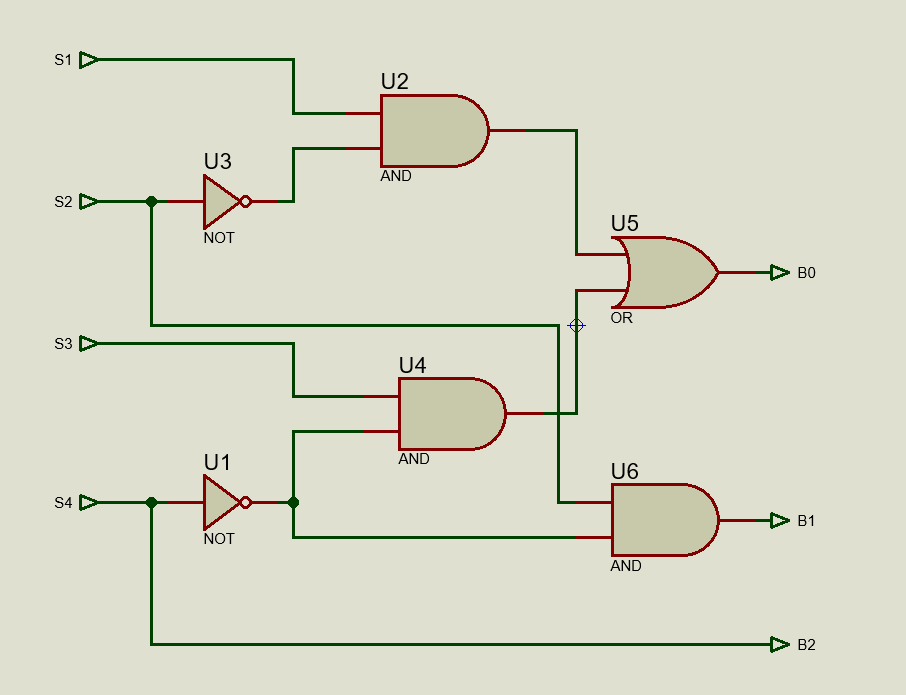
\includegraphics[width=0.92\textwidth]{img/encoder-interno.png}
  \caption{Implementación interna del codificador dentro del subcircuito ENCODER.}
\end{figure}

Para las pruebas conectamos generadores de estado lógico a cada uno de los
sensores, lo que nos permite simular las señas manualmente sin tener que armar
nada físico todavía.

\begin{figure}[H]
  \centering
  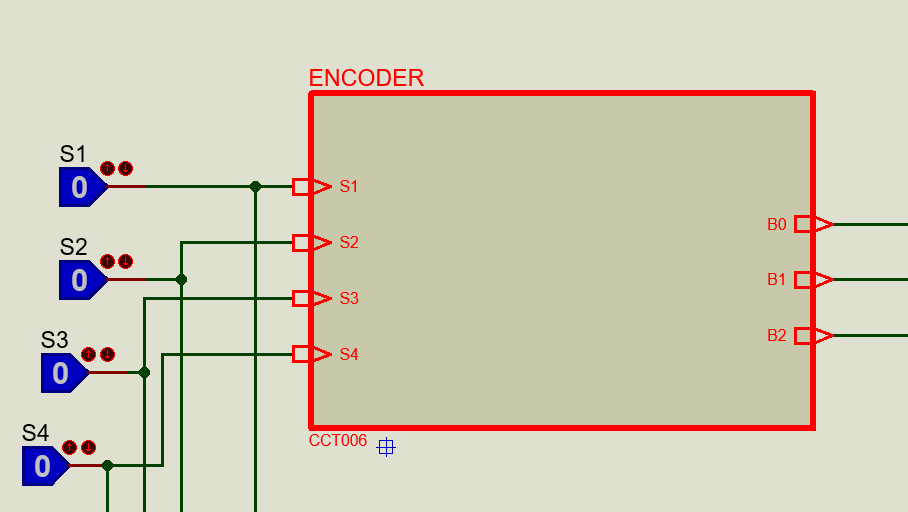
\includegraphics[width=0.85\textwidth]{img/encoder-bloque.png}
  \caption{Bloque ENCODER visto desde el esquemático principal, con los
  generadores de estado lógico usados para las pruebas.}
\end{figure}

Recorrimos las cinco señas válidas una por una y en todas la salida coincidió con
el valor esperado de la tabla de verdad, dado a que el circuito responde
correctamente pasamos a integrarlo con el resto del diseño.

\end{document}
